\section{Aufbau}
\label{sec:Aufbau}
Allen Messungen liegt ein einfacher Aufbau zu Grunde. An einer Beamline des Elektronenspeicherrings DELTA
wird die im davorliegenden elektromagnetischen Undulator entstehende, Strahlung über einen Spiegel 
ausgekoppelt. Diese wird über zwei weitere Spiegel in eine dunkle Box geleitet. Dort durchquert der 
Lichtstrahl zuerst eine Blende dann eine Reihe von neutrale Dichte Filtern und eine weitere Blende bevor 
er auf eien Photomultiplier trifft. Dort werden einzelne Phottonen in elektrische Pulse umgewandelt.
Diese Pulse werden im weiteren mit unterschiedlichen Messinstrumenten aufgezeichnet und später ausgewertet.
\subsection{Oszilloskop}
\label{sec:Oszilloskop}

\subsection{TDC7201}
\label{sec:TDC}
Beim TDC7201 handelt es sich um einen Time to Digital Converter. Dieser besitzt einen Eingang für ein 
Start Signal und einen Eingang für ein Stop Signal. Der Chip misst die Zeit zwischen den steigenden oder 
fallenden Flanken der Signale. Die gemessenen Zeiten können dann über einen SPI Bus ausgelesen werden.
Das geschieht in diesem Aufbau durch einen Raspberry Pi. Dieses Verfahren funktioniert in nahezu Echtzeit. 
Daher kann mit diesem Aufbauleicht eine Füllstruktur errechnet und über das EPICS Protokoll im Netzwerk 
zur verfügung gestellt werden. Als Startsignal wird der DELTA Umlauftrigger genutzt. Als Stopsignal wird 
das Signal des Photomultipliers genutzt. Da es bei diesem Aufbau wahrscheinlicher ist Photonen von Bunches 
zu messen die als erstes nach dem Umlauftrigger Signal kommen, sollte das Umlauftriggersignal nach jeder 
Messung um zwei Nannosekunden verzögert werden um so alle Bunches über die Zeit gleich gut vermessen zu können.
Dazu wurde der Delaygenerator über das VXII Protokoll vom Raspberry Pi angesteuert.
Dieses Vorhaben scheiterte jedoch daran das der Delaygenerator nicht schnell genug umschalten konnte.
Daher müssen die gemessenen Signale später rechnerisch korrigiert werden. Dazu wurde ein Histogramm über 
meherere Umläufe erstellt und anhand dessen der Abfall der Messwahrscheinlichkeit bestimmt.
\begin{figure}
  \centering
  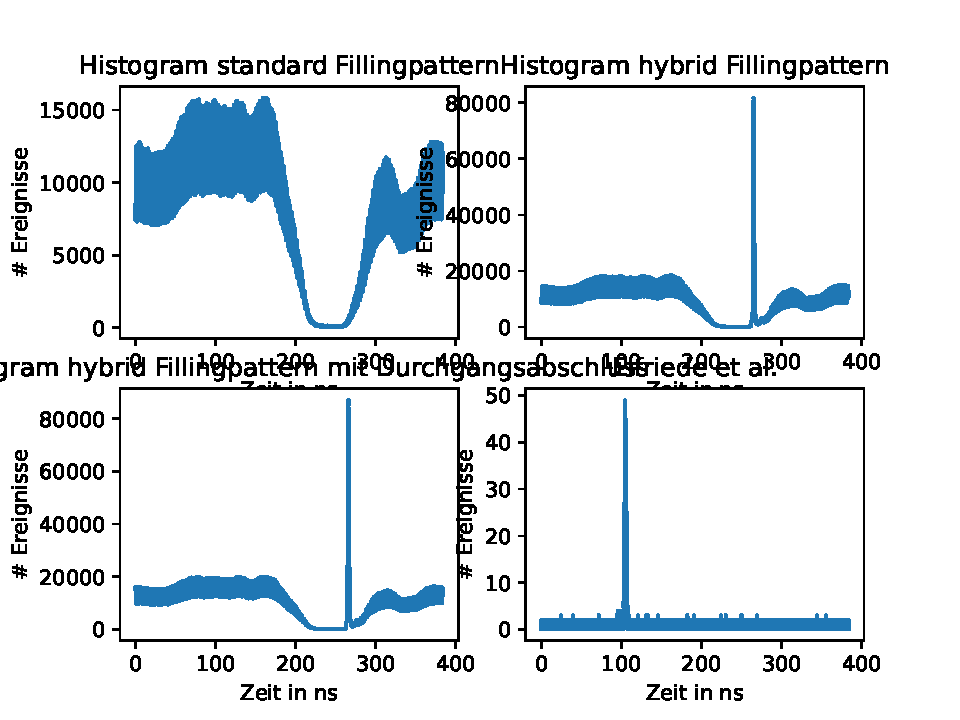
\includegraphics{content/plots/multiplot1.pdf}
  \caption{Plot.}
  \label{fig:plot}
\end{figure}


Siehe \autoref{fig:plot}!


\subsection{Time Tagger}
\label{sec:TimeTagger}
Der Time Tagger ist ein dem in \autoref{sec:TDC} beschriebenen Aufbau ähnliches kommerzielles Produkt
der Firma Swabian Instruments.